\section[Audioadapter]{Audioadapter \cite{da:sps}}
\label{sec:audioadapter}

Der Audioadapter wurde entwickelt, um Echtzeit Audioverarbeitung (Signalverarbeitung) mit dem ARM-\gls{Minimalsystem} zu ermöglichen. Die eingelesenen Audiosignale, die beispielsweise von einem Mikrofon geliefert werden, werden abgetastet und mit einem \gls{ADC} in einen digitalen Wert gewandelt und via \IIS{} zum Microcontroller gesendet. Dort werden sie dann verarbeitet. Schließlich wird das Audiosignal dann via \IIS{} zu einem \gls{DAC} gesendet und Schließlich wird das analoge Signal wieder auf einem Lautsprecher ausgegeben.

\subsection{Aufbau des neuen Audioadapters}
\subsubsection{Blockschaltbild}
Der Audioadapter besteht prinzipiell aus den Ein- und Ausgängen (Klinke und Cinch), aus einem Audiocodec und einem analogen Schalter (Analog Switch – TS5A22364). Mit dem Analog Switch kann zwischen den beiden Eingängen, Klinke und Cinch, gewählt werden. Dazu muss einfach der Auswahl-Jumper entsprechend umgesteckt werden. Der durchgeschaltete Eingang wird mit den analogen Eingängen (linker und rechter Kanal) des Audiocodecs TLV320AIC23B verbunden. Das analoge Signal wird mit einem \gls{ADC} in ein digitales Signal umgewandelt. Die genauere Funktion des Audiocodecs ist unter \fref{sec:audio-codec} erklärt. Nach dem \gls{DAC} erfolgt die Ausgabe auf beide Ausgänge.

Die Auswahl fiel auf den Audiocodec TLV320AIC23B weil dieser einen \enquote{Crystal Input} besitzt. Dadurch kann die Taktversorgung direkt auf dem Audioadapter durch einen \unit{12}{\mega\hertz} Quarz erfolgen. Außerdem gibt es einen fertigen VHDL-Code, der von Professor Hermann Dum geschrieben und zur Verfügung gestellt wurde, mit dem der Audiocodec über das FPGA-Board BASYS2 konfiguriert werden kann. Ein Entwicklungsmodul mit dem Audiocodec TLV320AIC23B wird auch im Labor verwendet. Dies erleichterte das Design der neuen Schaltung für den Audioadapter, die Testung des fertigen Audioadapters, so wie das Konfigurieren des Audiocodecs über \IIC{} mit dem \gls{ARM} \gls{Minimalsystem}.

\fig{audio-bsb}{Blockschaltbild der Audioplatine}{Blockschaltbild der Audioplatine}{\textwidth}{Schuh/Pictures/audio-bsb}

\subsubsection{Schematic}
In \fref{fig:audio-schem} sieht man die gesamte Schaltung des Audioadapters. Die einzelnen Funktionsblöcke werden in den nächsten Punkten genauer erklärt.

\fig{audio-schem}{Gesamtschematic der Audioplatine}{Gesamtschematic der Audioplatine}{0.75\textwidth}{Schuh/Pictures/audio-schem}

\subsubsection{Audio Codec TLV320AIC23B \cite{ti:tlv320aic23b}}
\label{sec:audio-codec}
Daten:
\begin{itemize}
    \item High Performance Stereo Codec
    \item \unit{90}{\deci\bel} \gls{SNR} Multibit Sigma-Delta \gls{ADC}
    \item \unit{100}{\deci\bel} \gls{SNR} Multibit Sigma-Delta \gls{DAC}
    \item Sample-Frequenz \unit{8}{\kilo\hertz} - \unit{96}{\kilo\hertz}
    \item 2-Wire SPI-compatible Serial-Port Protocols
    \item \IIS{}-compatible Interface
    \item Standard \IIS{}, \gls{MSb} or \gls{LSb} justified data transfer
    \item 16/20/24/32 bit Wortbreite
\end{itemize}

\fig{audio-codec-bsb}{Funktionsblockschaltbild des Audiocodec}{Funktionsblockschaltbild des Audiocodec \cite{ti:tlv320aic23b}}{\textwidth}{Schuh/Pictures/audio-codec-bsb}

Von den analogen Eingängen wurden nur LLINEIN und RLINEIN verwendet. Der Eingang MICIN ist unbelegt. Die Eingänge können getrennt durch softwareseitige Konfiguration der entsprechenden Register in \unit{1,5}{\deci\bel} Schritten von \unit{+12}{\deci\bel} bis \unit{-34}{\deci\bel} verstärkt bzw. abgeschwächt werden (\fref{fig:audio-codec-bsb}: grün markiert). Von den Ausgängen wurden nur die Headphone-Ausgänge verwendet. Diese können ebenfalls durch Konfiguration der entsprechenden Register verstärkt oder abgeschwächt werden. Dies ist in \unit{1}{\deci\bel} Schritten von \unit{+6}{\deci\bel} bis \unit{-73}{\deci\bel} möglich (\fref{fig:audio-codec-bsb}: blau markiert). Die Konfiguration wird über den Mode-Pin (Pin 22) nach \fref{tab:audio-codec-mode} festgelegt. 

\tab{audio-codec-mode}{Modi des Audiocodec}{Modi des Audiocodec \cite{ti:tlv320aic23b}}{|c|c|}{
    \hline
    \textbf{Mode} & \textbf{Interface}\\
    \hline
    0 & \IIC{}\\
    \hline
    1 & SPI\\
    \hline
}

Im SPI-Modus werden die Daten über SDIN (Pin 23) übertragen. SCLK (Pin 24) ist der serielle Takt. $\overline{CS}$ (Pin 21) wird \texttt{0} wenn die Übertragung eines Datenworts abgeschlossen ist.

\fig{audio-codec-spi}{SPI-Timing des Audiocodec}{SPI-Timing des Audiocodec \cite{ti:tlv320aic23b}}{0.75\textwidth}{Schuh/Pictures/audio-codec-spi}

Im \IIC{}-Modus werden die Daten über SDIN (Pin 23) übertragen und der serielle Takt über SCLK (Pin 24). $\overline{CS}$ (Pin 21) stellt die Adresse ein (\fref{tab:audio-codec-iic-addr}) und ist hardwaremäßig auf GND (\texttt{0}) geschaltet.

\tab{audio-codec-iic-addr}{\IIC{}-Adresse des Audiocodec}{\IIC{}-Adresse des Audiocodec \cite{ti:tlv320aic23b}}{|c|c|}{
    \hline
    \textbf{$\overline{CS}$} & \textbf{Adresse}\\
    \hline
    0 & \texttt{0011010}\\
    \hline
    1 & \texttt{0011011}\\
    \hline
}

\fig{audio-codec-iic}{\IIC{}-Timing des Audiocodec}{\IIC{}-Timing des Audiocodec \cite{ti:tlv320aic23b}}{0.75\textwidth}{Schuh/Pictures/audio-codec-iic}

Da der Mode-Pin bei der Audioadapterplatine hardwaremäßig auf \texttt{0} gelegt wurde, erfolgt die Konfiguration mit \IIC{} über das Control Interface (\fref{fig:audio-codec-bsb}: rot markiert). Die Audiodatenübertragung erfolgt im Digital Audio Interface über \IIS{} (\fref{fig:audio-codec-bsb}: gelb markiert). Da der Audiocodec bei unserer Anwendung im Master Modus arbeitet (kann im Register \enquote{Digital Audio Interface Format} konfiguriert werden), wird der Takt BCLK, LRCOUT und LRCIN vom Audiocodec erzeugt.

\fig{audio-codec-pinning}{Pinbelegung des Audiocodec}{Pinbelegung des Audiocodec \cite{ti:tlv320aic23b}}{0.75\textwidth}{Schuh/Pictures/audio-codec-pinning}

\FloatBarrier
\ltab{audio-codec-pins}{Pinbelegung des Audiocodec}{Pinbelegung des Audiocodec \cite{ti:tlv320aic23b}}{|c|c|p{10cm}|}{
    \hline
    \textbf{Name} & \textbf{Pin} & \textbf{Beschreibung}\\
    \hline
    AGND & 15 & Analog supply return\\
    \hline
    AVDD & 14 & Analog supply input. Voltage level is \unit{3,3}{\volt} nominal\\
    \hline
    BCLK & 3 & \IIS{} serial-bit clock. In master-mode: AIC23B generates signal; in slave-mode: DSP generates signal\\
    \hline
    BVDD & 1 & Buffer supply input, Voltage range is from \unit{2,7}{\volt} to \unit{3,6}{\volt}\\
    \hline
    CLKOUT & 2 & Clock output, buffered version of XTI input, 1x or 1/2x frequency\\
    \hline
    $\overline{CS}$ & 21 & Control port input latch/address select. SPI: data latch control/\IIC{}: address pin\\
    \hline
    DIN & 4 & \IIS{} format serial data input to the sigma-delta stereo \gls{DAC}\\
    \hline
    DGND & 28 & Digital supply return\\
    \hline
    DOUT & 6 & \IIS{} format serial data output from the sigma-delta stereo \gls{ADC}\\
    \hline
    DVDD & 27 & Digital supply input. Voltage range is \unit{1,4}{\volt} to \unit{3,6}{\volt}.\\
    \hline
    HPGND & 11 & Analog headphone amplifier supply return\\
    \hline
    HPVDD & 8 & Analog headphone amplifier supply input. Voltage level is \unit{3,3}{\volt} nominal.\\
    \hline
    LHPOUT & 9 & Left stereo mixer-channel amplified headphone output. Nominal \unit{0}{\deci\bel} output level is \unit{1}{\volt}$_{RMS}$. Gain of \unit{–73}{\deci\bel} to \unit{6}{\deci\bel} is provided in \unit{1}{\deci\bel} steps.\\
    \hline
    LLINEIN & 20 & Left stereo-line input channel. Nominal \unit{0}{\deci\bel} input level is \unit{1}{\volt}$_{RMS}$. Gain of \unit{-34,5}{\deci\bel} to \unit{12}{\deci\bel} is provided in \unit{1,5}{\deci\bel} steps.\\
    \hline
    LOUT & 12 & Left stereo mixer-channel line output. Nominal output level is \unit{1}{\volt}$_{RMS}$.\\
    \hline
    LRCIN & 5 & \IIS{} DAC-word clock signal. In audio master mode, the AIC23B generates this framing signal and sends it to the \gls{DSP}. In audio slave mode, the signal is generated by the \gls{DSP}.\\
    \hline
    LRCOUT & 7 & \IIS{} ADC-word clock signal. In audio master mode, the AIC23B generates this framing signal and sends it to the \gls{DSP}. In audio slave mode, the signal is generated by the \gls{DSP}.\\
    \hline
    MICBIAS & 17 & Buffered low-noise-voltage output suitable for electret-microphone-capsule biasing. Voltage level is 3/4 AVDD nominal.\\
    \hline
    MICIN & 18 & Buffered amplifier input suitable for use with electret-microphone capsules. Without external resistors a default gain of 5 is provided.\\
    \hline
    MODE & 22 & Serial-interface-mode input.\\
    \hline
    RHPOUT & 10 & Right stereo mixer-channel amplified headphone output. Nominal 0-dB output level is \unit{1}{\volt}$_{RMS}$. Gain of \unit{–73}{\deci\bel} to \unit{6}{\deci\bel} is provided in \unit{1}{\deci\bel} steps.\\
    \hline
    RLINEIN & 19 & Right stereo-line input channel. Nominal 0-dB input level is \unit{1}{\volt}$_{RMS}$. Gain of \unit{-34,5}{\deci\bel} to \unit{12}{\deci\bel} is provided in \unit{1,5}{\deci\bel} steps.\\
    \hline
    ROUT & 13 & Right stereo mixer-channel line output. Nominal output level is \unit{1}{\volt}$_{RMS}$.\\
    \hline
    SCLK & 24 & Control-port serial-data clock. For SPI and 2-wire control modes this is the serial-clock input.\\
    \hline
    SDIN & 23 & Control-port serial-data input. For SPI and 2-wire control modes this is the serial-data input and also is used to select the control protocol after reset.\\
    \hline
    VMID & 16 & Midrail voltage decoupling input. \unit{10}{\micro\farad} and \unit{0,1}{\micro\farad} capacitors should be connected in parallel to this terminal for noise filtering. Voltage level is 1/2 AVDD nominal.\\
    \hline
    XTI/MCLK & 25 & Crystal or external-clock input. Used for all internal clocks on the AIC23B.\\
    \hline
    XTO & 26 & Crystal output. Connect to external crystal when the AIC23B is the master\\
    \hline
}

\ltab{audio-codec-unusedpins}{Nicht benutzte Pins des Audiocodec}{Nicht benutzte Pins des Audiocodec \cite{ti:tlv320aic23b}}{|c|c|p{10cm}|}{
    \hline
    \textbf{Name} & \textbf{Pin} & \textbf{Beschreibung}\\
    \hline
    LOUT & 12 & \multirow{2}{10cm}{Die Ausgänge LOUT und ROUT wurden freigelassen, da nur die verstärkbaren/abschwächbaren Ausgänge LHPOUT und RHPOUT verwendet wurden.}\\
    \cline{1-2}
    ROUT & 13 &\vspace{1cm}\\
    \hline
    MICBIAS & 17 & \multirow{2}{10cm}{MICBIAS und MICIN wurden nicht beschaltet, da für unsere Anwendung nur 2 Eingänge gebraucht werden und der MIC-Eingang einen zusätzlichen Eingang benötigen würde.}\\
    \cline{1-2}
    MICIN & 18 &\vspace{1cm}\\
    \hline
    CLKOUT & 2 & Der CLKOUT (\unit{12}{\mega\hertz} bzw \unit{6}{\mega\hertz}) wird für keine Anwendung benötigt.\\
    \hline
}

\tabpdf{audio-codec-reg}{Register des Audiocodec}{Register des Audiocodec \cite{ti:tlv320aic23b}}{0.75\textwidth}{Schuh/Pictures/audio-codec-reg}

\subsubsection{Analog Switch TS5A22364 \cite{ti:ts5a22364}}
Der TS5A22364 ist ein bidirektionaler, analoger Schalter mit 2 Kanälen. Er wurde ausgewählt, da er im Gegensatz zu anderen analogen Schaltern keine negative Versorgungsspannung benötigt, um trotzdem negative Signale durchzulassen. Die maximale positive Spannung, die er durchlassen kann entspricht VCC, die maximale negative Spannung VCC – \unit{5,5}{\volt}. Das ergibt einen Durchlassbereich von \unit{+3,3}{\volt} bis \unit{-2,2}{\volt} und ist somit ausreichend für die Eingangssignale des Audioadapters.

\fig{audio-switch-pinning}{Pinbelegung des Analog Switch}{Pinbelegung des Analog Switch \cite{ti:ts5a22364}}{0.75\textwidth}{Schuh/Pictures/audio-switch-pinning}

\tab{audio-switch-pins}{Pinbelegung des Analog Switch}{Pinbelegung des Analog Switch \cite{ti:ts5a22364}}{|c|c|p{10cm}|}{
    \hline
    \textbf{Name} & \textbf{Pin} & \textbf{Beschreibung}\\
    \hline
    VCC & 1 & Power Supply\\
    \hline
    NO1 & 2 & Normally Open (NO) signal path, Switch 1\\
    \hline
    COM1 & 3 & Common signal path, Switch 1\\
    \hline
    NC1 & 4 & Normally Closed (NC) signal path, Switch 1\\
    \hline
    IN1 & 5 & Digital control pin to connect COM1 to NO1 or NC1, Switch 1\\
    \hline
    GND & 6 & Ground\\
    \hline
    IN2 & 7 & Digital control pin to connect COM2 to NO2 or NC2, Switch 2\\
    \hline
    NC2 & 8 & Normally Closed (NC) signal path, Switch 2\\
    \hline
    COM2 & 9 & Common signal path, Switch 2\\
    \hline
    NO2 & 10 & Normally Open (NO) signal path, Switch 2\\
    \hline
}

\fig{audio-switch-bsb}{Funktionsblockschaltbild des Analog Switch}{Funktionsblockschaltbild des Analog Switch \cite{ti:ts5a22364}}{0.75\textwidth}{Schuh/Pictures/audio-switch-bsb}

Die zwei Audioquellen auf der linken Seite stellen die Eingänge des Audioadapters (Klinke und Cinch) dar. Der Lautsprecher stellt den Ausgang dar, und wiedergibt je nach Input Select eine der beiden Audioquellen. Der interne Shunt Switch verhindert \enquote{Click and Pop} beim Umschalten zwischen den Audioquellen. Der Input Select wurde mit einem Jumper zum Wechseln zwischen GND und VCC realisiert. Welche Jumperstellung welchen Eingang durchschaltet ist auf dem Audioadapter beschrieben und wird hier nochmal mit den nächsten beiden Abbildungen dargestellt.

Die in \fref{fig:audio-switch-jmp-chinch} gezeigte Jumperstellung verbindet die miteinander verbundenen IN-Pins mit VCC und der Cincheingang wird durchgeschaltet.
Die in \fref{fig:audio-switch-jmp-klinke} gezeigte Jumperstellung verbindet die IN-Pins mit GND und der Klinkeneingang wird durchgeschaltet.

\begin{figure}[H]
    \centering
    \subfloat[Chinch\label{fig:audio-switch-jmp-chinch}]{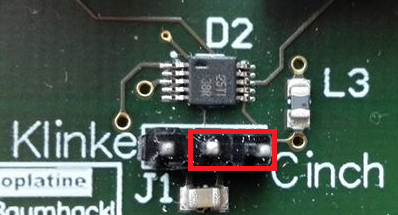
\includegraphics[width=.4\linewidth]{Schuh/Pictures/audio-switch-jmp-chinch}}\qquad
    \subfloat[Klinke\label{fig:audio-switch-jmp-klinke}]{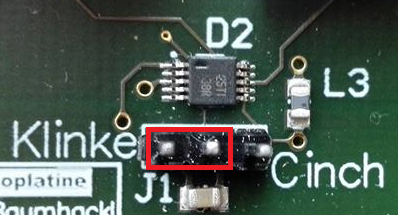
\includegraphics[width=.4\linewidth]{Schuh/Pictures/audio-switch-jmp-klinke}}\qquad
    \caption{Analog Switch Jumperpositionen}
    \label{fig:audio-switch-jmp}
\end{figure}

\fig{audio-switch-schem}{Schematic des Analog Switch}{Schematic des Analog Switch}{\textwidth}{Schuh/Pictures/audio-switch-schem}

\FloatBarrier
Zum Testen des analogen Switches wurde jeweils an einem Kanal der Cincheingänge und an einem Kanal des Klinkeneingangs ein Signal angelegt. Am Cincheingang liegt ein \unit{300}{\milli\volt} Sinussignal mit \unit{1}{\kilo\hertz} an (\fref{fig:audio-switch-oszi1}: gelbes, oberstes Signal). Am Klinkeneingang liegt ein \unit{300}{\milli\volt} Sinussignal mit \unit{2}{\kilo\hertz} an (\fref{fig:audio-switch-oszi1}: blaues, mittleres Signal).

\fig{audio-switch-oszi1}{Eingangssignale am Analog Switch}{Eingangssignale am Analog Switch}{0.75\textwidth}{Schuh/Pictures/audio-switch-oszi1}

Das Ausgangssignal ist in den folgenden Abbildungen als unterstes Signal beim Oszilloskop zu sehen. Die Eingangssignale schauen am Oszilloskop, vermutlich durch das Verwenden der T-Stücke am Frequenzgenerator, etwas verrauscht aus. Als erstes wurde der Jumper J1 auf \enquote{Chinch} umgesteckt.

\fig{audio-switch-oszi2}{Cincheingang am Analog Switch durchgeschaltet}{Cincheingang am Analog Switch durchgeschaltet}{0.75\textwidth}{Schuh/Pictures/audio-switch-oszi2}

Das Signal am Klinkeneingang wird über den internen Shunt Switch gegen Masse geschaltet. Das Signal vom Cincheingang wird durchgeschaltet und kommt am Ausgang wieder heraus, siehe \fref{fig:audio-switch-oszi2}. Danach wurde der Jumper auf \enquote{Klinke} umgesteckt.

\fig{audio-switch-oszi3}{Klinkeneingang am Analog Switch durchgeschaltet}{Klinkeneingang am Analog Switch durchgeschaltet}{0.75\textwidth}{Schuh/Pictures/audio-switch-oszi3}

Nun wurde das Signal am Cincheingang über den internen Shunt Switch gegen Masse geschaltet. Das Signal vom Klinkeneingang wird durchgeschaltet und kommt am Ausgang wieder heraus, siehe \fref{fig:audio-switch-oszi3}.

\subsubsection{Ein- und Ausgänge}
Es stehen zum Anschließen einer Audioquelle ein Cinch-Eingang und ein Klinken-Eingang zur Verfügung. Die Ausgabe erfolgt ebenfalls entweder über Cinch oder Klinke.

\begin{figure}[H]
    \centering
    \subfloat[Frontansicht\label{fig:audio-io-front}]{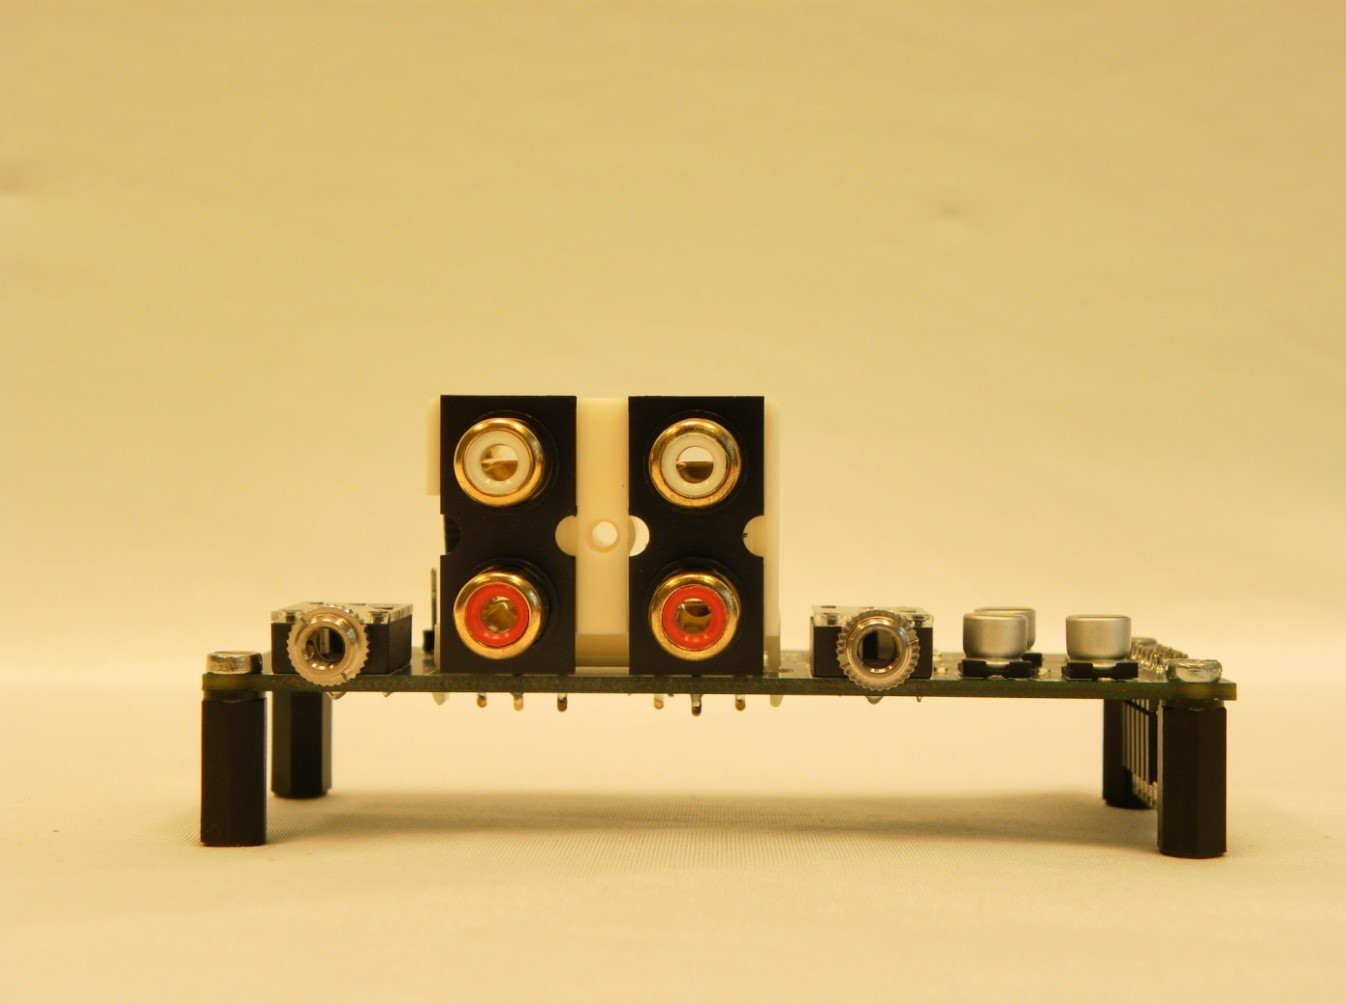
\includegraphics[width=.4\linewidth]{Schuh/Pictures/audio-io-front}}\qquad
    \subfloat[Draufsicht\label{fig:audio-io-up}]{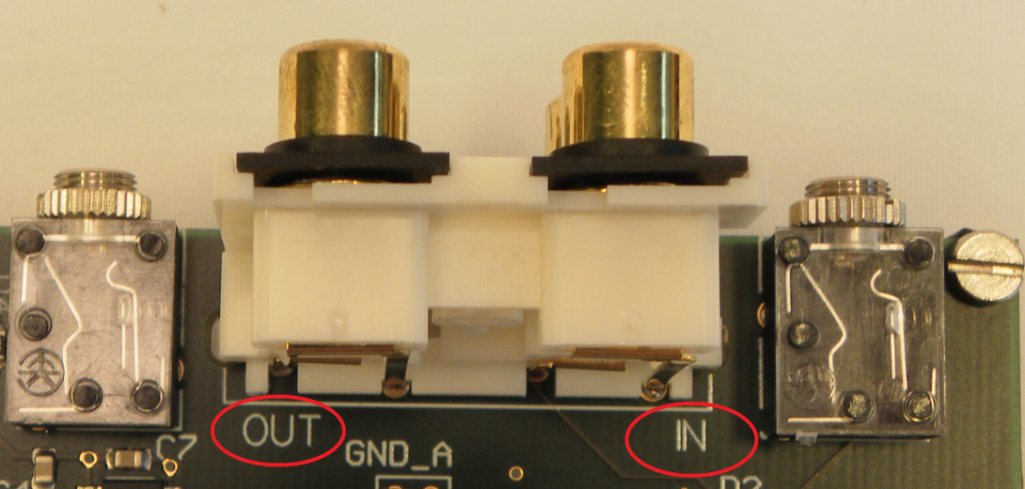
\includegraphics[width=.4\linewidth]{Schuh/Pictures/audio-io-up}}\qquad
    \caption{Audioplatine Ein- und Ausgänge}
    \label{fig:audio-io}
\end{figure}

Die Eingänge befinden sich in der Frontansicht (\fref{fig:audio-io-front}) auf der linken Seite und in der Draufsicht (\fref{fig:audio-io-up}) auf der rechten Seite. Sie sind auf der Platine zusätzlich mit \enquote{IN} beschriftet. Bei den Cinchbuchsen ist die rote Buchse der rechte Kanal und die weiße Buchse der linke Kanal.

Die Ausgänge befinden sich in der Frontansicht (\fref{fig:audio-io-front}) auf der rechten Seite und in der Draufsicht (\fref{fig:audio-io-up}) auf der linken Seite. Sie sind auf der Platine zusätzlich mit \enquote{OUT} beschriftet. Hier ist ebenfalls bei den Cinchbuchsen die rote Buchse der rechte Kanal und die weiße Buchse der linke Kanal.

\subsubsection{Schnittstelle zur \gls{Basisplatine}}
Der Audioadapter wird über die Schnittstelle (\fref{fig:audio-conn}: J2) mit der \gls{Basisplatine} verbunden. Die Spannungsversorgungen \unit{+3,3}{\volt} und \unit{+5}{\volt} werden von der \gls{Basisplatine} zur Verfügungen gestellt, wobei nur die \unit{+3,3}{\volt} verwendet werden.

\fig{audio-conn}{Schnittstelle zur Basisplatine}{Schnittstelle zur \gls{Basisplatine}}{\textwidth}{Schuh/Pictures/audio-conn}

\tab{audio-conn}{Schnittstelle zur Basisplatine}{Schnittstelle zur \gls{Basisplatine}}{|c|c|p{10cm}|}{
    \hline
    \textbf{Pin} & \textbf{NAme} & \textbf{Beschreibung}\\
    \hline
    1 & \unit{+5}{\volt} &\\
    \hline
    2 & \unit{+3,3}{\volt}D & Versorgung für Audiocodec und Analog Switch\\
    \hline
    3 & PB6 = I2C\_SCLK & \IIC{}1, SCLK-Leitung; Taktleitung von \IIC{}1-Interface + Pull-Up\\
    \hline
    4 & PB7 = I2C\_SDIN & \IIC{}1, SDIN-Leitung; Datenleitung von \IIC{}1-Interface + Pull-Up\\
    \hline
    5 & PA4 = I2S\_LRCIN & \IIS{}3, LRCIN; Left-Right-Clock-IN-Leitung von \IIS{}3-Interface\\
    \hline
    6 & PC10 = I2S\_BCLK & \IIS{}3, BCLK; Bit-Clock-Leitung von \IIS{}3-Interface\\
    \hline
    7 & PC12 = I2S\_DIN & \IIS{}3, SIN; Serial-Data-IN-Leitung von \IIS{}3-Interface\\
    \hline
    8 & PB12 = I2S\_LRCOUT & \IIS{}2, LRCOUT; Left-Right-Clock-OUT-Leitung von \IIS{}2-Interface\\
    \hline
    9 & PB13 = I2S\_BCLK & \IIS{}2, BCLK; Bit-Clock-Leitung von \IIS{}2-Interface\\
    \hline
    10 & PB15 = I2S\_DOUT & \IIS{}2, DOUT; Serial-Data-OUT-Leitung von \IIS{}2-Interface\\
    \hline
    11 & PC6 & Not connected\\
    \hline
    12 & DGND & Masse für den Audioadapter\\
    \hline
}

\begin{warning}
    Hinweis: Die Bezeichnungen sind immer aus der Sicht des Audiocodecs (bzw. des Audioadapters) beschrieben. I2S\_DIN sind also die Daten, die der Audiocodec \textbf{empfängt}.
\end{warning}

\subsubsection{Layout}
In \fref{fig:audio-layout} ist das fertige Layout und die Abmessungen der Platine dargestellt. Geroutet wurde nur am Toplayer (rot) und am Bottomlayer (blau). Die zwei inneren Layer der 4-fach Multilayer Platine sind eine Masse- und eine Versorgungsfläche, jeweils unterteilt in Digital- und Analogteil.

\fig{audio-layout}{Fertig geroutetes Layout}{Fertig geroutetes Layout}{\textwidth}{Schuh/Pictures/audio-layout}

\subsubsection{Trennung von digitalen und anlaogen Signalen}
Da der Audiocodec eine analoge und digitale Versorgung hat, sollten sowohl die Versorgungsspannung VCC von \unit{+3,3}{\volt}, als auch die Masse GND in einen digitalen und analogen Teil getrennt werden. Dadurch soll der Analogteil vom Digitalteil entkoppelt werden, um z.B. Störungen durch digitale Schaltvorgänge vom Analogteil fernzuhalten. Wichtig ist, dass der analoge Teil und der digitale Teil räumlich möglichst gut getrennt sind und die Massefläche bzw. die Versorgungsfläche möglichst durchgehend ist, was bei einer Multilayerplatine kein Problem darstellt. Außerdem sollten analoge Signale, also die Audiosignale, über dem analogen Teil geführt werden. Digitale Signale, wie z.B. verschiedene Takte und Steuersignale, sollten über dem digitalen Teil geführt werden.

\fig{audio-layout-trennung}{GND Layer unterteilt in Analog- und Digitalteil}{GND Layer unterteilt in Analog- und Digitalteil}{\textwidth}{Schuh/Pictures/audio-layout-trennung}
\fig{audio-layout-trennung2}{VCC Layer unterteilt in Analog- und Digitalteil}{VCC Layer unterteilt in Analog- und Digitalteil}{\textwidth}{Schuh/Pictures/audio-layout-trennung2}

Die GND- und VCC-Kupferflächen sind durch eine Unterbrechung getrennt. Die Unterbrechung wird in \fref{fig:audio-layout-trennung} von der grünen bzw. roten (\fref{fig:audio-layout-trennung2}) Linie, die quer durch die Platine verläuft, dargestellt. Die Layer-Einstellungen können in Altium Designer 14.3 unter \texttt{Design} $\rightarrow$ \texttt{Layer Stack Manager} vorgenommen werden.

\fig{audio-layout-trennung3}{Altium: Layer Stack Manager}{Altium: Layer Stack Manager}{\textwidth}{Schuh/Pictures/audio-layout-trennung3}

Im Layer Stack Manager (\fref{fig:audio-layout-trennung3}) sieht man die zwei Signal-Layer (Top Layer und Bottom Layer) und die zwei internen Flächen bzw. Internal Planes (GND-Plane und VCC-Plane).

Die analoge und digitale Versorgungsspannung wird normalerweise durch eine Spule bzw. durch eine Ferritperle an einem Punkt verbunden. Auch die analoge und digitale Masse wird getrennt und an einem Punkt verbunden. Es wurden dafür mehrere Stellen vorgesehen. Die Verbindung erfolgt durch das Einlöten eines 0 $\Omega$ Widerstands. Eventuell führt das Verwenden einer Ferritperle zu noch besseren Ergebnissen. An welcher Stelle und mit welchem Bauteil (0 $\Omega$ Widerstand oder Ferritperle) die Trennung zwischen Analogteil und Digitalteil zum besten Ergebnis führt, müsste durch Messen getestet werden, was allerdings nicht geschah.

\subsubsection{Bestückungsplan}
\fig{audio-best-top}{Bestückungsplan Top}{Bestückungsplan Top}{\textwidth}{Schuh/Pictures/audio-best-top}
\fig{audio-best-bottom}{Bestückungsplan Bottom}{Bestückungsplan Bottom}{\textwidth}{Schuh/Pictures/audio-best-bottom}

\subsubsection{Baugruppen}
In \fref{fig:audio-bau-schem} ist eine Übersicht der wichtigsten Baugruppen des Audioadapters dargestellt und in \fref{fig:audio-bau-schem} der fertigbestückte Audioadapter.

\fig{audio-bau-schem}{Übersicht Baugruppen}{Übersicht Baugruppen}{\textwidth}{Schuh/Pictures/audio-bau-schem}
\fig{audio-bau-bild}{Fertige Audioplatine}{Fertige Audioplatine}{\textwidth}{Schuh/Pictures/audio-bau-bild}

\subsubsection{Testen des Audioadapters mit dem FPGA Board Basys2}
Der erste Test des Audioadapters wurde mit dem FPGA Board Basys2 durchgeführt. Da es für diesen Audiocodec bereits eine fertige VHDL Anwendung gibt, musste nur noch eine Adapterplatine gelötet und die Ausgänge im \texttt{.ucf} File geändert werden.

\subsubsection{Basys2 Adapterplatine}
Um eine kompakte Adapterplatine zu löten wurden die benötigen Ein-/Ausgänge im \texttt{top\_audio\_proc1.ucf} File vom VHDL Projekt \enquote{audiocodec.xise} auf die ersten zwei Stecker (JA und JB) gelegt, siehe \fref{lst:audio-ucf}.

\lstinputlisting[language={VHDL}, caption=User-Constraints für audiocodec.xise, label=lst:audio-ucf]{Schuh/Listings/top_audio_proc1.ucf}

Die Adapterplatine wurde nachfolgender Schaltung gelötet, wobei hier nur die zwei relevanten Stecker (JA und JB) gezeichnet wurden.

\fig{audio-fpga-schem}{Schematic FPGA Adapterplatine}{Schematic FPGA Adapterplatine}{\textwidth}{Schuh/Pictures/audio-fpga-schem}

\subsubsection{Testaufbau}
\fig{audio-fpga-test}{Testaufbau mit FPGA Board}{Testaufbau mit FPGA Board}{0.75\textwidth}{Schuh/Pictures/audio-fpga-test}

Nach dem Einschalten des FPGA-Boards muss der Button \texttt{0} gedrückt werden, damit der Audiocodec initialisiert wird. Die Schalter \texttt{0} und \texttt{1} müssen für eine Verstärkung von \unit{0}{\deci\bel} beide auf \enquote{low} sein.

\subsubsection{Messergebnisse}
Zum Testen wurde an einem Kanal ein Sinus mit einer Frequenz von \unit{1}{\kilo\hertz} und einer Spannung von \unit{500}{\milli\volt}$_{pp}$ angelegt (\fref{fig:audio-mess-oszi1}: gelbes Signal). Der Audiocodec wurde so konfiguriert, dass die Verstärkung \unit{0}{\deci\bel} ist. Am Ausgang kommt wieder dasselbe Signal heraus (\fref{fig:audio-mess-oszi1}: blaues Signal).

\fig{audio-mess-oszi1}{Messung des Ein-/Ausgangssignal}{Messung des Ein-/Ausgangssignal}{0.75\textwidth}{Schuh/Pictures/audio-mess-oszi1}

Danach wurde die Verstärkung des Audiocodecs getestet. Dazu wurde der Schalter \texttt{0} auf \enquote{high} umgestellt. Beim erneuten Konfigurieren wurden die Register \enquote{left (\& right) line input channel volume control} auf eine Verstärkung von \unit{6}{\deci\bel} eingestellt. Das Ausgangssignal war doppelt so groß wie das Eingangssignal, siehe \fref{fig:audio-mess-oszi2}.

\fig{audio-mess-oszi2}{Messung der Verstärkung x2}{Messung der Verstärkung x2}{0.75\textwidth}{Schuh/Pictures/audio-mess-oszi2}

Außerdem wurde noch ermittelt, wie weit der \gls{DAC} vom Audiocodec aussteuern kann. Dazu wurde der Audiocodec so konfiguriert, dass die Verstärkung \unit{18}{\deci\bel}, also den Faktor 8 beträgt. Das Eingangssignal wurde nun so lange erhöht, bis das Ausgangsignal abgeschnitten wurde. Dies war bei einem Eingangssignal von \unit{450}{\milli\volt}$_{pp}$ der Fall. Das Ausgangssignal wurde erst bei etwa \unit{3,4}{\volt}$_{pp}$ abgeschnitten. Es kann also die gesamte Versorgungsspannung von \unit{3,3}{\volt} ausgenutzt werden, siehe \fref{fig:audio-mess-oszi3}.

\fig{audio-mess-oszi3}{Abgeschnittenes Ausgangssignal}{Abgeschnittenes Ausgangssignal}{0.75\textwidth}{Schuh/Pictures/audio-mess-oszi3}

\subsection{Testen der Audioadapterplatine am \gls{Minimalsystem}}
Beim Testen mit dem \gls{ARM} \gls{Minimalsystem} wurden sowohl die Cincheingänge (links und rechts), als auch der Klinkeneingang getestet. Als Eingang wurde ein Sinussignal mit \unit{500}{\milli\volt}$_{pp}$ mit einer Frequenz von \unit{1}{\kilo\hertz} eingespeist. Das Eingangssignal ist in \fref{fig:audio-mini-oszi} auf Kanal 1 (gelb) zu sehen. Das Ausgangssignal ist auf Kanal 2 (blau) zu sehen. Die Register wurden so konfiguriert, dass die Verstärkung \unit{0}{\deci\bel} (x1) beträgt. \fref{fig:audio-mini-oszi} zeigt die Messung, bei dem das Signal beim linken Cincheingang angeschlossen wurde und wieder am linken Cinchausgang gemessen wurde.

\fig{audio-mini-oszi}{Messung mit Minimalsystem}{Messung mit Minimalsystem}{0.75\textwidth}{Schuh/Pictures/audio-mini-oszi}

Die Messungen, bei denen das Signal bei einem anderen Eingang angeschlossen wurde, ergaben dasselbe Ergebnis.

\subsection{Messung der alten und neuen Audioplatine}
\subsubsection{Wichtige Eigenschaften von ADCs und DACs}
Im Folgenden werden wichtige Eigenschaften von \gls{ADC}s und \gls{DAC}s näher erläutert. Die Eigenschaften, die hier angeführt werden, wurden bei der \enquote{alten} und bei der \enquote{neuen} Audioplatine mit dem UPV-Audioanalyzer (\fref{sec:audio-messgerät}) gemessen.

\subsubsubsection{SNR - Signal to Noise Ratio}
Das Signal zu Rausch Verhältnis beschreibt das Verhältnis zwischen der RMS Amplitude des Ausgangssignals zur RMS Amplitude des Rauschens. Die ersten 9 harmonischen Schwingungen werden nicht in die Berechnung mit einbezogen.

\eq{audio-snr-1}{
    SNR = 20 * log(\frac{Signalleistung}{Rauschleistung})
}

Bei einer Signalamplitude von \unit{1}{\volt} und einer durchschnittlichen Rauschamplitude von \unit{1}{\milli\volt} würde das folgendes S/N Verhältnis ergeben:

\eq{audio-snr-2}{
    SNR = 20 * log(\frac{\unit{1}{\volt}}{\unit{1}{\milli\volt}}) = \unit{60}{\deci\bel}
}

Der ideale Signal zu Rausch Abstand lässt sich ungefähr mit folgender Formel berechnen, wobei n die Anzahl der Bit (Auflösung) angibt.

\eq{audio-snr-2}{
    SNR_{ideal} = \unit{6,02}{\deci\bel} * n - \unit{1,76}{\deci\bel}
}

\subsubsubsection{Klirrfaktor (THD - Total Harmonic Distortion)}
Die Total Harmonic Distortion (= gesamte harmonische Verzerrung) bzw. der Klirrfaktor beschreibt das Verhältnis der summierten Leistungen der Oberschwingungen zur Leistung der Grundschwingung.

\fig{audio-thd-schem}{reines Sinussignal}{reines Sinussignal}{0.75\textwidth}{Schuh/Pictures/audio-thd-schem}

Eine reine Sinusschwingung mit der Frequenz f1 ergibt folgendes das Spektrum, welches in \fref{fig:audio-thd-spec} zu sehen ist. Es ist nur die Frequenz f1 vorhanden und es gibt keine Oberschwingungen.

\fig{audio-thd-spec}{Spektrum ohne Harmonische}{Spektrum ohne Harmonische}{0.75\textwidth}{Schuh/Pictures/audio-thd-spec}

\fig{audio-thd-schem2}{Analog-Digital gewandeltes Sinussignal}{Analog-Digital gewandeltes Sinussignal}{0.75\textwidth}{Schuh/Pictures/audio-thd-schem2}

Wird das reine Sinussignal nun mit einem Analog-Digital Konverter umgewandelt (\fref{fig:audio-thd-schem2}) ergeben sich harmonische Schwingungen, die im Spektrum aussehen, wie in \fref{fig:audio-thd-spec2} gezeigt.

\fig{audio-thd-spec2}{Spektrum mit Harmonischen}{Spektrum mit Harmonischen}{0.75\textwidth}{Schuh/Pictures/audio-thd-spec2}

\FloatBarrier
Wie im vorherigen Spektrum ist wieder das Grundsignal f1 (in grün) zu erkennen. Die weiteren Frequenzen f2 bis f9 (in rot und gelb) sind harmonische Schwingungen. Zur Berechnung der THD werden allerdings nur die ersten 6 harmonischen Schwingungen (in rot) benötigt.

Allgemein werden nichtlineare Verzerrungen in Prozent (Klirrfaktor k) oder in dB (Klirrdämpfung ak) angegeben.

\eq{audio-thd-1}{
    THD = \frac{\sqrt{v^2(f_2) + v^2(f_3) + \dots + v^2(f_7)}}{v(f_1)}
}

Das Umrechnen von dB in Prozent bzw. von Prozent in dB erfolgt mit folgenden Formeln:

\eq{audio-thd-2}{
    k(\%) = 100 * 10^{\frac{a_k(dB)}{20}}
}

\eq{audio-thd-3}{
    a_{k}(dB) = 20 * \log_{10}(\frac{k(\%)}{100})
}

ak(dB) muss bei der Umrechnung als negativer Wert eingesetzt werden. Das Verhältnis zwischen Klirrfaktor und Klirrdämpfung wird in der folgenden Tabelle dargestellt.

\tab{audio-thd-ratio}{Verhältnis zwischen Klirrfaktor und Klirrdämpfung}{Verhältnis zwischen Klirrfaktor und Klirrdämpfung}{|c|c|}{
    \hline
    \textbf{Klirrfaktor [\%]} & \textbf{Klirrdämpfung [dB]}\\
    \hline
    100 & 0\\
    \hline
    10 & -20\\
    \hline
    1 & -40\\
    \hline
    0,1 & -60\\
    \hline
}

\subsubsubsection{SFDR - Spurious Free Dynamic Range}
SFDR (\enquote{störungsfreier dynamischer Bereich}) ist der Abstand der größten Störung zur Grundschwingung. Die größte Störung kann sowohl eine harmonische Schwingung (wie in der Abbildung dargestellt), als auch Rauschen sein. In \fref{fig:audio-sfdr} sieht man den störungsfreien dynamischen Bereich im Spektrum eingezeichnet.

\fig{audio-sfdr}{Spurious Free Dynamic Range}{Spurious Free Dynamic Range}{0.75\textwidth}{Schuh/Pictures/audio-sfdr}

\subsubsubsection{SINAD - Signal to Noise and Distortion}
SINAD ist eine Kombination aus den beiden vorherigen Eigenschaften, SNR und THD. Es beschreibt das Verhältnis zwischen der RMS Amplitude des Ausgangssignals zur RMS Amplitude aller anderen Pegel (Rauschen + Harmonische), ausgenommen Gleichspannung. SINAD wird in dB angegeben und kann mit folgender Formel berechnet werden.

\eq{audio-sinad}{
    SINAD = 20 * \log{\sqrt{10^{-\frac{SNR}{10}} + 10^{\frac{THD}{10}}}}
}

\subsubsubsection{ENOB - Effective Number of Bits}
ENOB beschreibt die tatsächliche Auflösung eines \gls{ADC}s bzw. \gls{DAC}s. Zum Beispiel kann ein \gls{ADC} mit 16 Bit Auflösung durch Verzerrungen und Rauschen eine tatsächliche Auflösung von nur 12 Bit haben.

Die ENOB kann aus der zuvor berechneten SINAD berechnet werden: 

\eq{audio-enob}{
    ENOB = \frac{SINAD - \unit{1,7}{\deci\bel}}{\unit{6,02}{\deci\bel}}
}

\subsubsection{Messgerät}
\label{sec:audio-messgerät}
Um die Qualität des alten und neuen Audioadapters zu vergleichen, wurden verschiedene Eigenschaften gemessen. Die Messungen wurden mit einem UPV Audioanalyzer von Rohde \& Schwarz durchgeführt.

\fig{audio-messgerat1}{UPV Audio Analyzer von Rhode \& Schwarz}{UPV Audio Analyzer von Rhode \& Schwarz}{0.75\textwidth}{Schuh/Pictures/audio-messgerat1}

Mit diesem Messgerät sind zahlreiche Audiomessungen möglich. Der Startbildschirm ist in \fref{fig:audio-messgerat2} dargestellt.

\fig{audio-messgerat2}{UPV Audio Analyzer Startbildschirm}{UPV Audio Analyzer Startbildschirm}{0.75\textwidth}{Schuh/Pictures/audio-messgerat2}

In den Fenstern \enquote{Generator Config} und \enquote{Generator Function} können die Einstellungen für das Signal, das beim Audioadapter eingespeist wird, eingestellt werden. Dazu gehören unter anderem die Spannung, die Frequenz, die Signalform und Funktionen wie Frequenzsweep. In den Fenstern \enquote{Analyzer Config} und \enquote{Analyzer Function} wird eingestellt, was gemessen werden soll und wie gemessen wird. Unter den Funktionen kann z.B. THD, SNR, FFT, SINAD und vieles mehr eingestellt werden. Außerdem können diverse Filter, wie z.B. das A-Weighting Filter, das bei der SNR Messung benötigt wurde, eingestellt werden. Im \enquote{Numeric Display} werden die Generatorspannung und das Messergebnis angezeigt. Die Messergebnisse können auch grafisch dargestellt werden, wie bei den folgenden Messergebnissen zu sehen ist.

\subsubsection{Messergebnisse des alten und neuen Audioadapters}
\label{sec:audio-messergebnisse}
In der Tabelle ist der Klirrfaktor des alten und des Audioadapters bei verschiedenen Eingangsspannungen vergleichbar. Die Messungen wurden bei einer Frequenz von \unit{1}{\kilo\hertz} durchgeführt. Die Eingangsspannung wurde bei dieser und allen folgenden Messungen von \unit{200}{\milli\volt}$_{RMS}$ bis \unit{900}{\milli\volt}$_{RMS}$ in \unit{100}{\milli\volt}-Schritten erhöht.

\tab{audio-messergebnisse-thd}{Messergebnisse Klirrfaktor}{Messergebnisse Klirrfaktor}{|c|c|c|c|c|}{
    \hline
    & \multicolumn{2}{|c|}{alter Audioadapter} & \multicolumn{2}{|c|}{neuer Audioadapter}\\
    \hline
    $U_{gen}$ [\milli\volt$_{RMS}$] & THD [dB] & THD [\%] & THD [dB] & THD [\%]\\
    \hline
    \hline
    200 & -29,4 & 9,687 & -77,7 & 0,013\\
    \hline
    300 & -28,8 & 10,160 & -77,9 & 0,013\\
    \hline
    400 & -29,5 & 9,611 & -76,8 & 0,014\\
    \hline
    500 & -29,4 & 9,687 & -77,0 & 0,014\\
    \hline
    600 & -28,4 & 10,488 & -79,5 & 0,011\\
    \hline
    700 & -28,3 & 10,572 & -81,4 & 0,009\\
    \hline
    800 & -28,4 & 10,488 & -83,4 & 0,007\\
    \hline
    900 & -27,8 & 11,000 & -83,9 & 0,006\\
    \hline
}

Normalerweise erhöht sich der Abstand zwischen der Grundschwingung und den harmonischen Schwingungen mit zunehmender Eingangsspannung (solange die Klippgrenze nicht erreicht bzw. überschritten wird). Bei den Ergebnissen des alten Audioadapters ist dies nicht der Fall. Der Klirrfaktor bleibt über den gesamten Eingangsspannungsbereich ähnlich. \fref{fig:audio-messergebnisse-thdold} ist der Klirrfaktor des alten Audioadapters bei einer Eingangsspannung von \unit{900}{\milli\volt}$_{RMS}$ mit einer Frequenz von \unit{1}{\kilo\hertz} grafisch dargestellt. Außerdem wird mit dem Marker der Abstand zur höchsten harmonischen Schwingung, also SFDR, markiert. In \fref{fig:audio-messergebnisse-thdnew} wird der Klirrfaktor des neuen Audioadapters bei der gleichen Eingangsspannung grafisch dargestellt. Außerdem wird wieder SFDR mit dem Marker angezeigt. Der Vergleich zeigt einen deutlich höheren Klirrfaktor des \enquote{alten} Audioadapters, verglichen mit dem \enquote{neuen} Audioadapter. Aus der vorherigen Messtabelle sind folgende Werte für THD bei einer Eingangsspannung von \unit{900}{\milli\volt}$_{RMS}$ zu entnehmen:

\tab{audio-messergebnisse-thd900}{Messergebnisse Klirrfaktor bei \unit{900}{\milli\volt}$_{RMS}$}{Messergebnisse Klirrfaktor bei \unit{900}{\milli\volt}$_{RMS}$}{|c|c|c|}{
    \hline
    $U_{gen}$ [\milli\volt$_{RMS}$] & THD alt [dB] & THD neu [dB]\\
    \hline
    900 & -27,8 & -83,9\\
    \hline
}

Die höchste Störung liegt beim \enquote{alten} Audioadapter bei \unit{2}{\kilo\hertz} nur \unit{28,243}{\deci\bel} unter der Grundschwingung, während beim \enquote{neuen} Audioadapter die größte Störung bei \unit{6}{\kilo\hertz} \unit{86,288}{\deci\bel} unter der Grundschwingung liegt.

\fig{audio-messergebnisse-thdold}{THD \& SFDR des alten Audioadapters ($U_{ein}$ = \unit{900}{\milli\volt})}{THD \& SFDR des alten Audioadapters ($U_{ein}$ = \unit{900}{\milli\volt})}{0.75\textwidth}{Schuh/Pictures/audio-messergebnisse-thdold}
\fig{audio-messergebnisse-thdnew}{THD \& SFDR des neuen Audioadapters ($U_{ein}$ = \unit{900}{\milli\volt})}{THD \& SFDR des neuen Audioadapters ($U_{ein}$ = \unit{900}{\milli\volt})}{0.75\textwidth}{Schuh/Pictures/audio-messergebnisse-thdnew}

\subsubsubsection{SNR}
In der Tabelle ist der Signal-zu-Rausch-Abstand des alten und neuen Audioadapters bei verschiedenen Eingangsspannungen gegenübergestellt. Die Frequenz, mit der gemessen wurde, beträgt \unit{1}{\kilo\hertz}. Außerdem wurde ein A-Weighting Filter verwendet, der beim UPV Audioanalyzer im Fenster \enquote{Analyzer Function} eingestellt wurde.

\tab{audio-messergebnisse-snr}{Messergebnisse Signal-Rausch-Abstand}{Messergebnisse Signal-Rausch-Abstand}{|c|c|c|}{
    \hline
    & alter Audioadapter & neuer Audioadapter\\
    \hline
    $U_{gen}$ [\milli\volt$_{RMS}$] & SNR [dB] & SNR [dB]\\
    \hline
    200 & 71,3 & 69,4\\
    \hline
    300 & 74,7 & 69,4\\
    \hline
    400 & 76,9 & 75,7\\
    \hline
    500 & 78,6 & 77,4\\
    \hline
    600 & 80,1 & 79,2\\
    \hline
    700 & 81,4 & 80,1\\
    \hline
    800 & 82,7 & 81,7\\
    \hline
    900 & 84,0 & 82,5\\
    \hline
}

Bei den Ergebnissen ist zu erkennen, dass der Signal-zu-Rausch-Abstand bei der alten Audioplatine minimal besser ist. Mit der Analyzer Funktion FFT ist in den folgenden zwei Abbildungen das Spektrum dargestellt. Im Spektrum sind sowohl die harmonischen Schwingungen, als auch das Rauschen zu sehen.

\fig{audio-messergebnisse-snrold}{FFT des alten Audioadapters ($U_{ein}$ = \unit{900}{\milli\volt})}{FFT des alten Audioadapters ($U_{ein}$ = \unit{900}{\milli\volt})}{0.75\textwidth}{Schuh/Pictures/audio-messergebnisse-snrold}
\fig{audio-messergebnisse-snrnew}{FFT des neuen Audioadapters ($U_{ein}$ = \unit{900}{\milli\volt})}{FFT des neuen Audioadapters ($U_{ein}$ = \unit{900}{\milli\volt})}{0.75\textwidth}{Schuh/Pictures/audio-messergebnisse-snrnew}

\subsubsubsection{SINAD \& ENOB}

\tab{audio-messergebnisse-enob}{Messergebnisse SINAD \& ENOB}{Messergebnisse SINAD \& ENOB}{|p{0.13\textwidth}|p{0.13\textwidth}|p{0.13\textwidth}|p{0.13\textwidth}|p{0.13\textwidth}|p{0.13\textwidth}|p{0.13\textwidth}|}{
    \hline
    & \multicolumn{3}{|c|}{alter Audioadapter} & \multicolumn{3}{|c|}{neuer Audioadapter}\\
    \hline
    $U_{gen}$ [\milli\volt$_{RMS}$] & SINAD [dB] gemessen & SINAD [dB] berechnet & ENOB berechnet & SINAD [dB] gemessen & SINAD [dB] berechnet & ENOB berechnet\\
    \hline
    \hline
    200 & 22,2 & 29,4 & 3 & 68,7 & 68,80 & 11\\
    \hline
    300 & 25,8 & 28,8 & 4 & 69,8 & 68,83 & 11\\
    \hline
    400 & 22,3 & 29,5 & 3 & 70,1 & 73,20 & 11\\
    \hline
    500 & 22,9 & 29,4 & 3 & 72,3 & 74,19 & 11\\
    \hline
    600 & 22,3 & 28,4 & 3 & 74,5 & 76,34 & 12\\
    \hline
    700 & 22,9 & 28,3 & 3 & 76,0 & 77,69 & 12\\
    \hline
    800 & 22,9 & 28,4 & 3 & 77,0 & 79,46 & 12\\
    \hline
    900 & 23,8 & 27,8 & 3 & 77,8 & 80,13 & 12\\
    \hline
}

In der Tabelle ist SINAD gemessen und berechnet zu sehen. Auf Grund der hohen harmonischen Störungen beim alten Audioadapter ergibt sich für SINAD ein schlechter Wert. Außerdem wurde aus SINAD die effektive Bitanzahl (ENOB) berechnet. Dieser Wert muss abgerundet werden (z.B. 12,5 Bit $\rightarrow$ 12 Bit). Dies würde beim alten Audioadapter theoretisch ein ENOB von 3 bis 4 ergeben, da sich die harmonischen Störungen stark auf die Berechnung auswirken. Dieser Wert ist allerdings nicht realistisch, da man diese geringe Auflösung beim Signal im Zeitbereich wahrnehmen würde (stufenförmiges Signal). Die ENOB des neuen Audioadapters ergibt einen Wert von 11 bzw. 12 ab einer Eingangsspannung von \unit{600}{\milli\volt}$_{RMS}$. Dieser Wert ist durchaus realistisch.
